\chapter{Theory: Neural dynamics}
\label{chap:Neuron}
\index{Multicompartmental neuron model}
Extracellular potentials \ehtxt{measured in neural tissue} are largely \tvnnote{vaere mer bastante her?} generated by the electrical activity of neurons. 
To model extracellular potentials, we therefore first need to model neurons. Neural modeling is a core topic in computational neuroscience, and has been covered in several text books in much greater detail than we intend to include in this one (see e.g.,\cite**{johnston1994foundations,KockSegev1998,Koch1999,DeSchutter2000,Hille2001,Dayan2005,Izhikevich2007,Sterratt2011,Miller2018}) 

Frameworks exist for constructing neuronal models at various levels of detail and abstraction. However, a neuron's contribution to the extracellular potential depends strongly on its morphology, \gex{in fact point-neuron models do not generate an extracellular potential at all.
Thus to model such potential}, we need to use \textit{multicompartmental} (MC) neuron models. The most common MC modeling framework
combines a so-called \textit{Hodgkin-Huxley type} description of the neural membrane mechanisms (see e.g., \cite**{Hodgkin1952,KockSegev1998,Pospischil2008}) with cable theory to predict how signals propagate spatially in dendrites and axons (see, e.g., \cite**{Koch1999,rall2011}). This framework has become the gold standard for biophysically detailed neuronal simulations on the cellular and network level, and has been used for simulating the dynamics of large neuronal networks (see e.g., \cite**{traub2005,markram2015,billeh2020} \gex{Billeh et al, Neuron, 2020}).  We will here only present this standard framework, which we will refer to simply as the MC framework. 

A\gex{n} MC model is characterized by (i) its morphology, and (ii) its membrane mechanisms, and the key dynamical variable is the membrane potential ($V$). The morphology (i) of the real neuron (\fref{fig:Neuron:multicomp}A) is represented as a discretized set of compartments connected by resistors (\fref{fig:Neuron:multicomp}B). There are two categories of currents which together determine the membrane potential dynamics in the compartments (\fref{fig:Neuron:multicomp}C). These are the currents that run intracellularly between compartments (yellow arrows), and the transmembrane currents in each compartment (green arrows), which are determined by a set of (ii) neuron specific membrane mechanisms. Once all the currents are characterized, the dynamics of the membrane potential can be computed by Kirchhoff's current law, which demands that the sum of currents into a given compartment is zero.\tvnnote{Hoeres ut som alle strommer regnes ut foerst, uavhengig av membranpotensialet? Kanskje vi ikke trenger dette avsnittet?}
\ehnote{et eller annet sted her savner jeg et statement ala "The spatiotemporal dynamics of the neuron are described in terms of sets of  partial differential equations derived from the electrical properties of the neuron. 
Effectively, the MC formalism allows for treating the neuron model and geometry as en equivalent electric circuit of capacitors, batteries and (voltage-dependent) resistors" (litt langt kanskje :/). 
Saann det leser naa, er morfologien det avgjoerende elementet.}
\gen{Jeg synes i grunn teksten til Geir var "barebones", klar og fin her :-)}

\begin{figure}[!ht]
\begin{center}
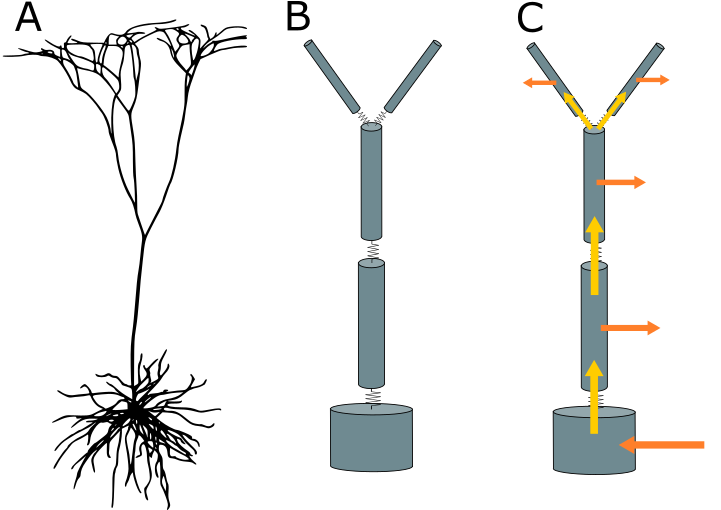
\includegraphics[width=0.6\textwidth]{Figures/Neuron/multicompartment.png}
\end{center}
\caption{\textbf{Multicompartmental modelling.}  (A) The neural morphology is (B) represented by a multicompartmental model, where the compartments are treated as cylinders connected by resistors. The example shows a crudely simplified model containing only five compartments, but detailed multicompartment models may include several hundreds of compartments, and can represent t he morphology in great detail. (C) Electric currents in the model can be separated into two groups: (i) transmembrane current in a compartment (green arrows), and (ii) intracellular currents between compartments (yellow arrows). 
}
\label{fig:Neuron:multicomp}
\end{figure}

Below, we first present a framework for modeling the transmembrane currents in a single compartment in \fref{sec:Neuron:membranecurrents}, and then go on to show how a number of such compartments can be connected together to a MC model in \fref{sec:Neuron:morphology}. Together, those two sections provide a theoretical framework for modeling neurons that should be sufficient for most practical applications. Readers that crave further biophysical insight into the ionic movements that mediate the transmembrane neural currents can get a brief introduction to this in \fref{sec:Neuron:Ions_and_reversals}. Finally, we end the chapter about neuronal modeling by briefly summarizing the main assumptions underlying the MC framework (\Fref{sec:Neuron:HHCassumptions}).


\section{\blue{Membrane currents}}
\label{sec:Neuron:membranecurrents}
\index{Hodgkin-Huxley type model}
Hodgkin-Huxley (HH) type models are called so because they describe the membrane mechanisms with a mathematical formalism similar to that used in celebrated model by \citeasnoun**{Hodgkin1952}. In HH-type models, the membrane typically includes three autonomous classes of transmembrane currents, normally represented as current densities (units \si{\milli\ampere\per\square\centi\metre}). These are (i) a capacitive current density ($i_{\mathrm{cap}}$), (ii) a leakage current density ($i_{\mathrm{L}}$), and (iii) a current density through active ion channels ($i_x$), of which there may be several different kinds ($x$ is an index). In addition, a neuron may receive (iv) external stimuli ($i_{\mathrm{stim}}$) either through synaptic currents or experimental current injections. 
\ehnote{Bedre symbol er $i_{\mathrm{ext}}$ for stroembidrag fra baade elektroder, synapser etc.}
\gen{Kanskje ikke optimalt aa kalle synaptisk input for et eksternt sitmulus her i boka?}

In the case where the neuron is modeled as a single compartment, the transmembrane currents into that compartment must sum to zero, so that:
\begin{equation}
i_{\mathrm{cap}}+ i_{\mathrm{L}} + \sum_x{i_x} +  i_{\mathrm{stim}} = 0.
\label{eq:Neuron:singlecomp_zerosum}
\end{equation}
Below, we define the various currents that go into this equation.

\subsection{\blue{Capacitive current}}
\label{sec:Neuron:Cap}
\index{Capacitive current}
The capacitive current density,
\begin{equation}
i_{\mathrm{cap}}= c_{\mathrm{m}} \frac{dV}{dt},
\label{eq:Neuron:HHcap}
\end{equation}
represents the charging up of \gex{the membrane to a} potential $V$ due to a charge density accumulating on the outside and inside of the capacitive membrane. 
\ehnote{I mine oerer skjaerer "charging up" noe. Kan vi ikke skrive "... represents the accumulation of charge in- and outside of the capacitive membrane as function of change in membrane potential $V$ over time."?} \gen{Dette gaar vel delvis paa valg av skrivestil? Jeg synes vi skal bruke saa enkle ord og skrive saa enkelt som mulig, og "charging up" er vel ikke galt? Og det h{\o}res enkelt, ujaalete og bra ut i mine {\o}rer.} 
Here, $c_{\mathrm{m}}$ is the \textit{specific membrane capacitance} defined as capacitance per membrane area. In the original HH model, $c_{\mathrm{m}}$ had the value 1 \si{\micro \farad / \cm}$^2$, and this value seems to be representative for most neurons.  An illustration of how to interpret the capacitive current is given in \fref{fig:Neuron:capacitive_currents}. 

\begin{figure}[!ht]
\begin{center}
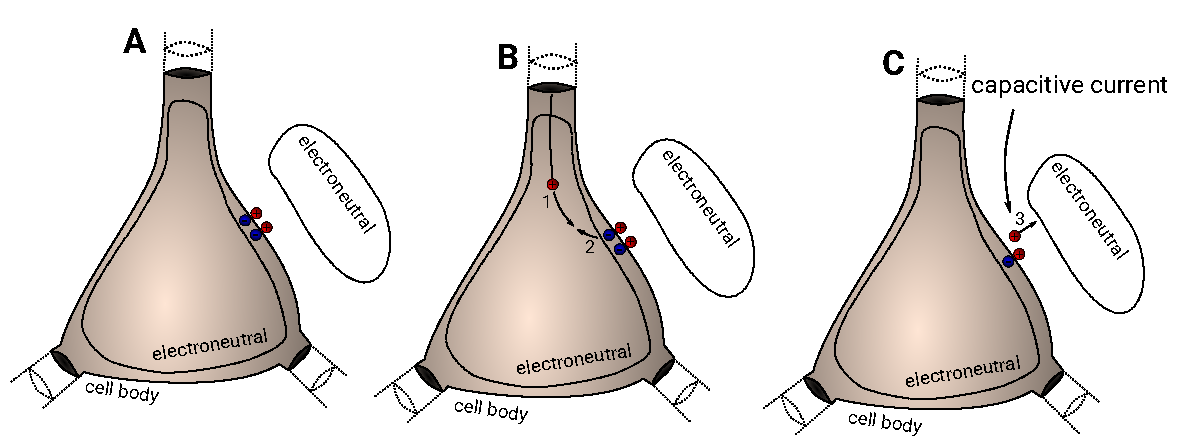
\includegraphics[width=1.0\textwidth]{Figures/Neuron/capacitive_currents.pdf}
\end{center}
\caption{\textbf{Capacitive currents are important for current \ehnote{"charge conservation" er et mer fundamentalt begrep} conservation.}  \gen{Ja, "charge conservarion" gjelder vel alltid, men her er vel poenget at dette leder til "current conservation" i vaart spesialtilfelle?} (\textbf{(A)}) The extracellular and intracellular bulk solutions are essentially electroneutral, and the only region where there is a nonzero charge density, is in thin Debye layers around the capacitive membrane. Unlike the other currents involved, the capacitive current is not due to ions crossing the membrane, but due to ions piling up on either side of it, separating a membrane charge density $\eta$ and a charge membrane charge density $-\eta$, giving rise to a membrane potential of $V = \eta/c_{\mathrm{m}}$. \gen{Det er vel ogsaa et lite str{\o}mbidrag 
fra "gating currents" i membranen, dvs. fra bundne ladninger som flytter paa seg, ikke at vi trenger aa komme inn paa det her.} An outward capacitive current could correspond to an anion leaving the membrane on the inside (\textbf{(B)}), which will coincide with a cation leaving the membrane on the outside (\textbf{(C)}). Thus, capacitive membrane currents do give rise to electrical ionic volume currents both in the intra- and extracellular space.
}
\label{fig:Neuron:capacitive_currents}
\end{figure}

If we insert \fref{eq:Neuron:HHcap} into \fref{eq:Neuron:singlecomp_zerosum}, we get:
\begin{equation}
c_{\mathrm{m}} \frac{dV}{dt} = - (i_{\mathrm{L}} + \sum_x{i_x} +  i_{\mathrm{stim}}),
\label{eq:Neuron:singlecomp_capinserted}
\end{equation}
which gives us an intuitive understanding of neurodynamics: If the sum of ionic currents over the membrane (right hand side) is nonzero, it will lead to a charging up (left hand side) of the membrane. \tvntxt{In other words, if for example positive ions are crossing the membrane and entering the cell (ionic current), this positive current will be exactly balanced by positive ions leaving the outside of the membrane because the cell has become less negative (capacitive current).}


\subsection{\blue{Leakage current}}
\label{sec:Neuron:leak}
\index{Leakage current}
The leakage current density is given by
\begin{equation}
i_{\mathrm{L}} = \bar{g}_{\mathrm{L}} (V - E_{\mathrm{L}}),
\label{eq:Neuron:HHleak}
\end{equation}
where $\bar{g}_{\mathrm{L}}$ (mS/cm$^2$) is the leak conductance (the bar indicates that it's a constant). 
\ehnote{Trengs virkelig den overline notasjonen? Lite konsekvent med andre parametre som ogsaa kun er skalarverdier. Veit det er brukt i HH-52-artikkelen, men virker litt utypisk i matte/fysikk ellers\ldots}
\gen{Tror det er ganske standard for aa betegne max-verdien til konduktanser, f.eks., brukt i Sterratt}
The factor $(V - E_{\mathrm{L}})$ (\si{\milli\volt}) is often called the driving force, \gen{driving force i italic?} and $E_{\mathrm{L}}$ the leak reversal potential\index{Reversal potential}. The biophysical origin of the reversal potential is explained later (see \fref{sec:Neuron:Ions_and_reversals}). For now, we may simply think of $E_{\mathrm{L}}$ as the "target potential" that the leakage current will strive to drive the membrane potential towards. In reality, the leakage current is not a single current, but represents an orchestra of physiological processes that together will drive the membrane potential towards the value $E_{\mathrm{L}}$. 

Together, the capacitive current and the leakage current determine the passive properties of the membrane. If the neuron were to include only these two currents, it could be well modeled as an RC-circuit, and RC-neuron\index{RC-neuron} models are often used to simulate the subthreshold dynamics of neurons (\Fref{fig:Neuron:RC}). 

\begin{figure}[!ht]
\begin{center}
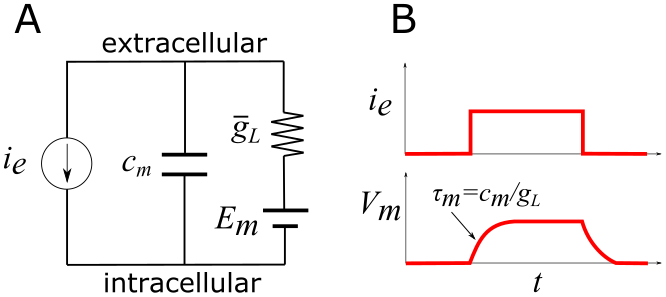
\includegraphics[width=0.8\textwidth]{Figures/Neuron/RCneuron.png}
\end{center}
\caption{\textbf{RC-neuron.}  A neuron model containing only a capacitive and a leakage current can be represented as an RC-circuit. To use standard MC modeling convention, we have expressed the various variables and parameters in units per membrane area: With a total membrane resistance $R = 1/(g_{\mathrm{L}} A)$, and capacitance $C = c_{\mathrm{m}}A$, we get that $RC = c_{\mathrm{m}}/g_{\mathrm{L}}$. In the illustration, the neuron is given an (electrode) injection $i_{\mathrm{e}}$ (A/cm$^2$) and responds by charging up the membrane. When the input is terminated, the membrane potential will return to the value $E_{\mathrm{L}}$. In the RC-model, $E_{\mathrm{L}}$ will be identical to the resting potential of the neuron, i.e., the potential that the membrane will settle on in the case where it does not receive any input. In models which include additional, active ion channels, these can in principle affect the resting potential, so that it may generally differ from $E_{\mathrm{L}}$.
}
\label{fig:Neuron:RC}
\end{figure}


\subsection{\blue{Active ion channels}}
\label{sec:Neuron:active}
\index{Ion channels! Voltage gated}
In addition to $i_{\mathrm{cap}}$ and $i_{\mathrm{L}}$, biophysical neuronal models include a number of active ion channels. These account for the fancy aspects of neurodynamics, 
\ehnote{"fancy" er vel kanskje litt upresist\ldots}
\gen{synes det er baade presist og l{\o}dig :-)}
and the main legacy of Hodgkin and Huxley was that they derived a mathematical model for describing the kinetics of these \cite**{Hodgkin1952}.

In the HH-type formalism, the current through an active ion channel type $x$ is modeled as:
\begin{equation}
i_x = \bar{g}_x m_x^{\alpha} h_x^{\beta}(V-E_x).
\label{eq:Neuron:HHform}
\end{equation}
We note that the current density $i_x$ does not represent the current through a single ion channel, but a large number of channels of the same type $x$. Thus, $\bar{g}_x$ (\si{\milli\siemens\per\square\centi\metre}) denotes the conductance when all channels of type $x$ are fully open (the bar indicates that it's a constant),
\tvnnote{Jeg ble fortalt en gang at dette ikke noedvendigvis var sant, og at parameterne kunne vaere slik at $m$ og $h$ aldri kunne naa 1, men husker ikke helt hva dette handlet om.}
\ehnote{Sannsynlighet for aapning/lukking som disse variablene representerer er kun paa intervallet $\langle 0, 1 \rangle$}
 while $E_x$ (\si{\milli\volt}) is the reversal potential for the ion species that travels through the channel type. In analogy with the leak reversal potential, we may think of $E_x$ as the target potential that the current through ion channel $x$ will strive to drive the membrane potential towards. The intrinsic membrane potential dynamics is thus due to the competition between various currents that all try to drive it towards their respective reversal potentials. 

If one prefers to think of neurons in terms of circuit diagrams, the active ion channels are simply added in parallel to the passive $i_{\mathrm{cap}}$ and $i_{\mathrm{L}}$ currents. As an example, the electric circuit representation of the HH model is depicted in \Fref{fig:Neuron:HH}.

\begin{figure}[!ht]
\begin{center}
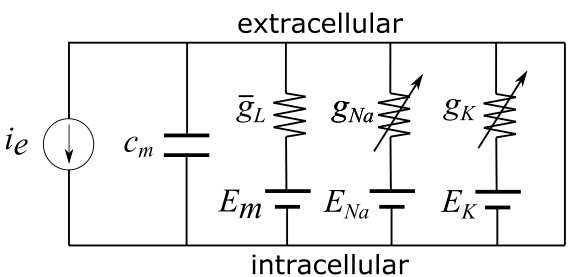
\includegraphics[width=0.8\textwidth]{Figures/Neuron/HHmodel.png}
\end{center}
\caption[]{\textbf{Active, single compartment neuron model.}  In addition to a capacitive and a leakage current, active neuron models contain a number of active ion channels. The example diagram shows the original Hodgkin-Huxley model, with an active Na$^+$ and an active K$^+$ channel. The arrows slicing the diagram conductances indicate that they are variables.}
\label{fig:Neuron:HH}
\end{figure}

Active ion channels differ from the passive leakage channel in that their total conductance, $\bar{g}_{x} m^{\alpha} h^{\beta}$, vary with time due to the so-called gating variables, in \fref{eq:Neuron:HHform} denoted $m$ and $h$\index{Gating variables}. These determine how the ion channels activate or deactivate (open or close), and $m$ and $h$ represent two different types of gates differing in terms of their opening/closing dynamics. The exponents $\alpha$ and $\beta$ represent the number of copies that a channel $x$ has of each type of gate. At the level of a single ion channel the values of $m$ and $h$ would interpret as the \textit{probability} that a given gate is in the open state. However, when we deal with summed currents through a large number of ion channels, the values of $m$ and $h$ interpret as the \textit{fraction} of the gates of the various types that are open. The values are thus numbers between 0 (all gates in the closed state) and 1 (all gates in the open state). The product $m^{\alpha} h^{\beta}$ thus interprets as the fractions of ion channels in which all gates are open so that currents can pass through. The ion channel conductance is thus given by the product $\bar{g}_x m_x^{\alpha} h_x^{\beta}$.

For voltage-gated ion channels, the the dynamics of the gating variables can be described by kinetics equations on the form:
\begin{equation}
\frac{dx(V,t)}{dt} = \frac{x_{\infty}(V) - x}{\tau_x(V)},  \, \text{for } x = \{m,h\}.
\label{eq:Neuron:HHgate}
\end{equation}
\ehnote{$x \in \{m, h\}$ siden $x$ er et diskret element i settet.}
Here, the steady state activation $x_{\infty}(V)$, represents the fraction of gates that will end up in the open state if the cell is clamped at a given potential $V$ for sufficiently long time. However, the process of opening the gates takes some time, as accounted for by the activation time constant $\tau_x(V)$ (\si{\milli\second}). Both $x_{\infty}(V)$ and $\tau_x(V)$ are functions of the membrane potential, and these must be determined experimentally for each individual ion channel type. We do not go into the experimental challenges here, but will think of them as known functions. 

There are also many ion channels whose activation or inactivation do not depend on $V$, but on some other variable, such as the concentration of some ion species or ligand \cite**{Hille2001,Sterratt2011}. A common example are Ca$^{2+}$ gated ion channels, i.e., channels with gate opening controlled by the intracellular Ca$^{2+}$ concentration ($\mathrm{[Ca^{2+}]_i}$). There are also ion channels whose activation depend on more than one variable, such as e.g., ion channels whose activation depend on both $V$ and $\mathrm{[Ca^{2+}]_i}$. A HH-type formalism can in most cases be applied also to these kind of ion channels, provided that $x_{\infty}(V)$ and $\tau_x(V)$ in \fref{eq:Neuron:HHgate} can be replaced with experimentally determined functions of the relevant variables \cite**{Sterratt2011}.

To give an example of an active neuron model, the full set of equations for the HH model is summarized in Box \ref{box:Neuron:HH}. Compared to modern biophysically detailed neuron models, the original HH model is relatively simple in that it only contains two (voltage-gated) active ion channels, a Na$^+$ with three activation gates ($m^3$) and one inactivation gate ($h$), as well as a K$^+$ channel with four inactivation gates $n^4$. The two active ion channels are together responsible for action potential generation.  

\begin{floatingbox}[h]
\caption{Hodgkin-Huxley equations}

\begin{eqnarray*}
    c_{\mathrm{m}} \frac{dV}{dt} & =  & -\bar{g}_{\mathrm{L}}(V-E_{\mathrm{L}}) - \bar{g}_{\mathrm{Na}} m^3 h (V - E_{\mathrm{Na}}) - \bar{g}_{\mathrm{K}} n^4 (V - E_{\mathrm{K}}) \\
    \frac{dx(V,t)}{dt} & = & \frac{x_{\infty}(V) - x}{\tau_x(V)},  \, \text{for } x = \{m,h,n\} \\ 
    x_{\infty}(V) &= & \frac{\alpha_x(V)}{\alpha_x(V) + \beta_x(V)}, \, \text{for } x = m,n,h \\ %\hline
    \tau_x(V) & = & \frac{1}{\alpha_x(V) + \beta_x(V)}, \, \text{for } x = m,n,h \\ %\hline
    \alpha_n &=& \frac{0.01 \mathrm{ms}^{-1} V+55\,\si{\milli\volt}}{1-e^{-(V+55\,\si{\milli\volt})/10\,\si{\milli\volt}}}  \\ %\hline
     \beta_n &=& 0.125 \mathrm{ms}^-1 e^{-(V+65\,\si{\milli\volt})/80\,\si{\milli\volt}}   \\ %\hline
     \alpha_m &=& \frac{0.1 \mathrm{ms}^{-1} V+ 40\,\si{\milli\volt}} {1-e^{-(V+40\,\si{\milli\volt})/10\,\si{\milli\volt}}}  \\   
     \beta_m &=& 4 \mathrm{ms}^{-1} e^{-(V+65\,\si{\milli\volt})/18\,\si{\milli\volt}}  \\ %\hline
    \alpha_h &=& 0.07 \mathrm{ms}^{-1} e^{-(V+65\,\si{\milli\volt})/20\,\si{\milli\volt}}  \\ %\hline
    \beta_h &=& \frac{1 \mathrm{ms}^{-1}}{1+e^{-(V+35\,\si{\milli\volt}))/10\,\si{\milli\volt})}}   \\ %\hline
    c_\mathrm{m} &=& 1.0 \,\si{\micro\farad\per\square\centi\metre} \\ %\hline
    \bar{g}_{\mathrm{Na}} &=& 120 \,\si{\milli\siemens\per\square\centi\metre}\\ %\hline
    \bar{g}_{\mathrm{K}} &=& 36 \,\si{\milli\siemens\per\square\centi\metre} \\ %\hline
    \bar{g}_{\mathrm{L}} &=& 0.3 \,\si{\milli\siemens\per\square\centi\metre} \\ %\hline
    E_{\mathrm{Na}} &=& 50 \,\si{\milli\volt} \\ %\hline
    E_{\mathrm{K}} &=& -77  \,\si{\milli\volt} \\ %\hline
    E_{\mathrm{L}} &=& -54.4 \,\si{\milli\volt} \\ %\hline
\end{eqnarray*}
\label{box:Neuron:HH}
\end{floatingbox}
\gen{Trenger en referanse inne i HH-boksen}
\gen{Vanskelig aa lese ligningene for $\alpha$ og $\beta$ - HH-boksen}

\ehnote{Burde ikke andre formalismer som termodynamiske og stokastiske (Markov?) modeller nevnes? HH formalismen er vel kun en empirisk approksimasjon som ikke ivaretar fundamentale fysiske prinsipp (energibevaring for eksempel).}



\subsection{\blue{Stimulus currents and synapses}}
\label{sec:Neuron:stim}
\index{Stimulus currents}
The stimulus current in \fref{eq:Neuron:singlecomp_zerosum} can represent any external stimulus that a neuron receives. Typically, it is either taken to represent an experimental electrode injection or a synaptic input. Below we include some typical examples of stimuli used in neuron simulations. 

\subsubsection{Current injections}
An electrode injection such as a step-current injection is modeled as:
\begin{equation}
i_\text{e}(t)= 
\begin{cases}
    constant, & \text{if } t_{start} < t < t_{end} \\
    0,              & \text{otherwise},
\end{cases}
\label{eq:Neuron:injected}
\end{equation}
\ehnote{$\text{for } t \in [t_\mathrm{start}, t_\mathrm{end}]$ - en annen ting er vel at oftest representeres disse punkt-stroemmene med enhet ampere, saa symbol $I_\mathrm{e}$}
Of course, one may chose the stimulus to be any function of time.


\subsubsection{Conductance-based synapses}
\index{Synapse}
\label{sec:Ch-Neuron:conductance-based-synapses}
A chemical synapse can be modeled more or less like an ion channel:
\begin{equation}
i_\text{syn}(t) = {g}_\text{syn}(t) \big(V(t)-E_\text{syn} \big), 
\label{eq:Neuron:chemicalsynapse}
\end{equation}
where $g_\text{syn}(t)$ is the synaptic conductance and $E_\text{syn}$ is the reversal potential of the synapse. 
\ehnote{jeg er litt forvirra, er synaptic conductance per areal eller ikke? Enhet S vs. S~m$^{-2}$? Jeg tenker synapser er punktprosesser uten romlig utstrekning saa enhet S og derfor notasjon $I_\mathrm{syn}, G_\mathrm{syn}$ Schuetter bruker liten bokstav av en eller annen grunn.}

The value of $E_\text{syn}$ determines whether the synapse is \textit{excitatory}, which means that it will tend to drive the  membrane potential of neuron toward the threshold for generating action potentials, or \textit{inhibitory}, which means that it will tend to drive the neuron away from the threshold for generating action potentials. Examples of excitatory synapses are AMPA and NMDA synapses, in which $E_\text{syn}$ ($\sim$ 0 \gex{--} 10 mV) is high above the neuronal resting potential. The most common inhibitory synapse is the GABA synapse, in which $E_\text{syn}$ ($\sim$ -70 mV) is close to the resting membrane potential of the neuron.

The synapse model described by \fref{eq:Neuron:chemicalsynapse} is called \textit{conductance based}, because the activation of the synapse is modeled as a transient change in the synaptic conductance. Unlike for ion channels, which are often voltage or calcium activated, the chemical synapse is activated by neurotransmitters received from a pre-synaptic cell. However, the synaptic response tends to be rather stereotypical, meaning that the post-synaptic conductance change is more or less the same every time the synapse is activated \tvnnote{Har vi kilde paa dette? Er dette egentlig sant? Har jo STD, STP osv. Swadlow 2002 for eksempel finner jo ganske andre resultater}. 
It is therefore not common to model neurotransmitter activation explicitly, but instead just
model $g_\text{syn}(t)$ as a constant $\bar{g}_\text{syn}$ multiplied with a temporal kernel determining the opening and closing of a synapse set off at an activation time $t_s$:
\begin{equation}
i_\text{syn}(t) = \bar{g}_\text{syn} f(t) \big(V(t)-E_\text{syn} \big).
\label{eq:Neuron:chemicalsynapse}
\end{equation}
Typical choices for $f(t)$ are\index{Synapse models}: 
\begin{align}
&\text{(i) exponential decay:} \;\; f(t) = e^{-(t-t_\text{s})/\tau}\, \Theta(t-t_\text{s}) \\
&\text{(ii) $\alpha$-function:} \;\; f(t) =  \frac{t-t_\text{s}}{\tau} e^{-(t-t_\text{s})/\tau} \, \Theta(t-t_\text{s}) \\
&\text{(iii) $\beta$-function:} \;\; f(t) = \frac{\tau_1 \tau_2}{\tau_1-\tau_2} 
\Big( e^{-(t-t_\text{s})/\tau_1} - e^{-(t-t_\text{s})/\tau_2} \Big) \, \Theta(t-t_\text{s}) \\
& \text{(iv) NMDA-like:} \;\; f(t) = \frac{e^{-(t-t_\text{s})/\tau_1} - e^{-(t-t_\text{s})/\tau_2}} {1+\mu [\text{Mg}^{2+}] e^{-\gamma V} } \, \Theta(t-t_\text{s}),
\label{eq:Neuron:sf4}
\end{align}
where $\Theta(t)$ is the (Heaviside) unit step function: $\Theta(t \ge 0)=1$,  $\Theta(t< 0)=0$, and where parameters like $\gamma$,  $\tau$, $\tau_1$ and $\tau_2$ must be tuned to experimental data from the particular synapse type that one wants to model. Simple waveform (cf., (i)--(iii) above) typically used for AMPA  and GABA synapses, while the waveform (iv), is mainly relevant for NMDA-synapses, where the conductance is influenced by membrane voltage and concentration of extracellular magnesium. 

The strength or efficacy of synaptic transmission may change over time through various processes that are often grouped together under the term "synaptic plasticity". Synaptic plasticity work as a mechanism for learning and memory formation in the brain. It is a much studied topic that has been treated in several text books (see e.g., \citeasnoun**{Joel1993} or \citeasnoun**{Kreutz2012}). We will not go further into this topic here.


\subsubsection{Current-based synapses}
\label{sec:Ch-Neuron:current-based-syn}
Currents through conductance-based synapses depend on the driving force, $V(t)-E_\text{syn}$ (\fref{eq:Neuron:chemicalsynapse}). A simpler synapse model is the current-based synapse, which rests on the assumption that the driving force $V(t)-E_\text{syn}$ can be approximated by a constant. The synaptic current then becomes:
\begin{equation}
i_\mathrm{syn}(t) = \overline{i}_\mathrm{syn} f(t), 
\label{eq:Neuron:CurrentBasedSynapse}
\end{equation}
where (cf. \fref{eq:Neuron:chemicalsynapse}):
\begin{equation}
\bar{i}_\mathrm{syn}=\bar{g}_\mathrm{syn}(\langle V(t) \rangle_t -E_\mathrm{syn}),
\label{eq:Neuron:CurrentBasedAvg}
\end{equation}
and where $\langle V(t) \rangle_t$ denotes the temporal average of the membrane potential. The temporal kernel
$f(t)$ can have the same exponential waveforms (i)-(iv) as the conductance based synapses. 
\ehnote{Jeg tenker subfix $t$ kan droppes siden $V(t)$ er 1D}

Unlike conductance-based synapses, current-based synapses are independent of the state ($V(t)$) of the neuron, and synaptic events thus become independent of previous synaptic events, something that facilitates the derivation of analytical solutions \cite**{Richardson2004,Cavallari2014}. Their relative simplicity have made current-based synapses popular in large network simulations because they reduce the computational load. 
\tvnnote{Should mention that they are linear}
\ehnote{Jeg tenker det er mer til det enn dette - for NEURON sin del er det lite aa hente paa lineariserte synapser siden MC formalismen krever numerisk integrasjon uansett - for punktnevroner med linear subthreshold dynamics (LIF etc.) kan man bruke eksakt integrasjon som er kjapt (i NEST for eksempel).}

\ghnote{Jeg skrev ikke mer enn det som staar over. Er det tilstrekkelig? Jeg ser at Espen har lagt inn noen kommentarer under, men trenger vi aa gaa inn paa disse tingene her? Espen, kan du se paa det, skrive inn noe ekstra om du mener det skal inn dit, og fjerne kommentarene hvis ikke?}

\ghnote{Man kunne jo skrevet flere sider om denne approksimasjonen, men jeg vet ikke hvor dypt vi vil gaa inn i dette.Jeg har ikke DeSchutter-boka, men har en hunch om at vi kan referere til den her. Er lite erfaren med bruk av slike synapser, og vet ikke hva de relevante referanser er. Espen - har du noe du vil legge til?}
\ehnote{Tok bort referansen til Hagen2016. Vi utleda ingen "closed-form solutions" der for dette. Vaart valg av synapsemodell var hentet direkte fra synapsemodellen i Potjans\&Diesmann2014. LIF punkt-nevroner med stroembaserte synapser kan loeses eksakt uten numerisk integrasjon og er populaert i kontekst av NEST for eksempel. Naa har vel andre studier som Roessert2016 (https://arxiv.org/abs/1604.00087) for eksempel vist at man kan approksimere effekten av dendrittisk kabel og synapsetroem med et ekvivalent filter, som implisitt resulter i en stroembasert "synapse" saa vidt jeg husker.}

\subsubsection{Gap-junctions}
\tvnnote{Brukes dette senere i boka? Hvis ikke kan vi kanskje ta det bort for enkelhets-skyld?}
\ehnote{Jeg ville beholdt dette - gap junctions er "vanlige". Om vi bruker de er en annen ting ;)}
In addition to the chemical synapses, some neurons also form electrical synapses called \underline{gap junctions}. A gap junction is basically an electric coupling between a branch of one neuron (with membrane potential $V_1$) and a branch of another neuron (with membrane potential $V_2$). The current through the gap junction is then simply the synaptic conductance multiplied with the voltage difference between the coupled branches:

\begin{equation}
i_\text{gap}=g_\text{gap} (V_{\mathrm{m}2}-V_{\mathrm{m}1}).
\label{eq:Neuron:gapjunction}
\end{equation}



%%%%%%%%%%%%%%%%%%%%%%%%%%
\section{\blue{Morphology}}
\label{sec:Neuron:morphology}
\index{Multicompartmental neuron model}
When we above introduced the various membrane currents, we mostly pictured the neuron as being a single compartment. In doing that, we implicitly assumed that the whole neuron was isopotential (same $V$ everywhere). 
\ehnote{Ikke aner jeg hvorfor det refereres til at antagelsen er 'isopotential compartments' - spesielt siden dette ville resultert i null aksialstroem og null transmembran stroem. For vaart formaal er vel en antagelse om tilnaermet konstant transmembran stroemtetthet langsmed hvert compartment langt bedre! Se foeroevrig kap 4.1.2 og kap 5.2.4.1 i NEURON-boka, potensialet til et kompartment er kun gyldig midt paa.}
However, in neurons with long and branchy dendrites, $V$ in the soma can be completely different from $V$ in the tip of a distal dendrite. If we want to account for the spatial aspect of neuronal signaling, we need to use multicompartmental (MC) models, where the neural morphology is represented as cylindrical compartments connected with resistors, and $V$ can be computed in each individual compartment (\Fref{fig:Neuron:multikompisen}A). 

\begin{figure}[!ht]
\begin{center}
\includegraphics[width=0.7\textwidth]{Figures/Neuron/multikompis.png}
\end{center}
\caption{\textbf{Multi-compartment model.} {\bf (A)} Representations of a neuronal morphology as a number of interconnected compartments. {\bf (B)} Subset of interconnected compartments. The currents involved in MC modeling include the sum of transmembrane currents ($I_{\mathrm{m},n}$) in a compartment $n$, and the intracellular currents running between 
compartments, $I_{n-1,n}$ (current from compartment $n-1$ to $n$), and $I_{n,n+1}$ (current from compartment $n$ to $n+1$).
}
\label{fig:Neuron:multikompisen}
\end{figure}

As a simple introduction to the formalism used in MC models, let us consider a subset of three connected cylindrical compartments which we number $n-1$, $n$ and $n+1$ (\Fref{fig:Neuron:multikompisen}B). For simplicity, we assume that the three cylinders have the same length ($L$) and diameter ($d$). The two categories of currents that run in this system are (i) the transmembrane currents that we introduced in the previous subsection, all of which we for now can group together into a total transmembrane current $I_{\mathrm{m},n}$, and (ii) the axial currents running between the cylindrical compartments ($I_{n-1,n}$ and $I_{n,n+1}$). The dynamics of this system is computed using Kirchhoff's current law, which demands that the sum of currents into a given compartment ($n$) should be zero:
\begin{equation}
I_{n-1,n} - I_{n,n+1} - I_{\mathrm{m},n} = 0.
\label{eq:Neuron:Kirch}
\end{equation}
We note that we here work with total currents (units \si{\ampere}), not current densities, so that $I_{\mathrm{m},n}$ is the sum of all current densities in the left hand side of \fref{eq:Neuron:singlecomp_zerosum} multiplied with the membrane area of compartment $n$. 

The axial current between two compartments is proportional to the voltage difference between the compartments, as determined by Ohm's law:
\begin{eqnarray}
I_{n-1,n} = \frac{V_{n-1}-V_n}{4 R_\text{a} L/(\pi d^2)}, \nonumber \\ 
I_{n,n+1} = \frac{V_{n}-V_{n+1}}{4 R_\text{a} L/(\pi d^2)}.
\label{eq:Neuron:axialcurrents}
\end{eqnarray}
Here, the denominators represent the axial resistance between two compartments, defined in terms of the axial resistivity $R_\text{a}$ (\si{\ohm\centi\metre}), a material property of the cytosol solution, the cross-section area, $\pi d^2/4$, and the segment length or travel distance, $L$ (\si{\metre})\tvnnote{Er L i meter?}. 

The calculations become more complicated when the connected cylinders are of different length and diameter, and especially at branch points. However, the theory for computing the dynamics in branching structures with varying diameters is well established \cite**{Rall1977,Rall1989}, and designated software such as NEURON \cite**{Hines1997,Hines2009} automatizes the compartmentalization for the user once the neural morphology is specified. For the reminder of this chapter, we limit ourselves to consider the simplified, unbranched scenario (\Fref{fig:Neuron:multikompisen}B), as we deem this as sufficient for establishing an understanding of the essentials of morphology\tvnnote{MC?} modeling. 

We note that in \fref{eq:Neuron:axialcurrents}, $V_n$ is the \emph{intracellular} potential in compartment $n$. However, in MC models, the intracellular potential is assumed to be identical to the membrane potential. This amounts to assuming that the extracellular resistivity is zero, so that the extracellular space is isopotential and grounded ($V = 0$ there) \tvnnote{Kan kanskje si: This amounts to assuming that any changes in the extracellular potential along the cell are small enough to have a negligible effect on the neural activity.}. This may seem like a peculiar assumption to make in a book where the extracellular potential is the main topic. We comment further on this assumption and its consequences at the end of this chapter. For now, we simply note that although the extracellular potential in reality is not zero, it is generally so much smaller than the intracellular potential that we can assume that it is zero without going too wrong when computing the neurodynamics. 


%%%%%%%%%%%%
\subsection{\blue{Active multicompartment models}}
\label{sec:Neuron:Active_multicomp}
To specify our MC neuron model further, we write out the total membrane current as:
\begin{equation}
I_{\mathrm{m},n} = I_{\mathrm{cap},n} + I_{\mathrm{ion},n} + I_{\mathrm{stim},n} = -\pi d L c_\text{m} \frac{dV_n}{dt} + \pi d L i_{\mathrm{ion},n} + I_{\mathrm{stim},n}
\label{eq:Neuron:Imemb}
\end{equation}
where $I_{\mathrm{ion},n}$ represents the total transmembrane ionic currents through leakage and active ion channels. In the last step, we expressed the capacitive and ionic currents (\si{\milli\ampere}) as current densities (\si{\milli\ampere\per\square\centi\metre}) multiplied with the membrane area ($\pi d L$ (\si{\square\centi\metre})) represented by the sides of the cylinder, and we have inserted \fref{eq:Neuron:HHcap} for the capacitive current density. If we insert this into \fref{eq:Neuron:Kirch}, we get the fundamental equation for multicompartmental models:

\begin{equation}
c_\text{m} \frac{dV_n}{dt} = i_{\mathrm{ion},n} + \frac{d}{4R_\text{a}}\left(\frac{V_{n+1}-V_n}{L^2} - \frac{V_n-V_{n-1}}{L^2} \right) + \frac{i_{\mathrm{stim},n}}{\pi d L}.
\label{eq:Neuron:multimain}
\end{equation}
\Fref{eq:Neuron:multimain} assumes that a compartment $n$ has two neighbors ($n-1$ and $n+1$), which will not be true for the endpoint compartments. To solve it, we must therefore select appropriate boundary conditions for these compartments. Common boundary conditions are those of a sealed end, where $\frac{\partial V_n}{\partial x} = 0$ for $n$ at the endpoints, or a killed end, where $V_n=0$ for $n$ at the endpoints. The NEURON simulator by default uses the sealed-end condition, which means that no axial current leaves at the endpoints of the simulated structure. 


%%%%%%%%%%%%%%%%%
\subsection{\blue{Passive multicompartment models}}
\label{sec:Neuron:Passive_multicomp}
\index{Multicompartmental neuron model}
If the neuron contains no active ion channels, $i_{\mathrm{ion},n} = g_\text{L}(V_n - E_L)$ is simply the leakage current density, and $E_L$ becomes identical to the membrane resting potential. It is then common to denote it by $E_\text{m}$, and to replace the leak conductance $g_\text{L}$ with the membrane resistivity $R_\text{m} = 1/g_\text{L}$ (\si{\ohm\square\centi\metre}). \Fref{eq:Neuron:multimain} then simplifies to:

\begin{equation}
c_\text{m} \frac{dV_n}{dt} = \frac{E_\text{m}-V_n}{R_\text{m}} + \frac{d}{4R_\text{a}}\left(\frac{V_{n+1}-V_n}{L^2} - \frac{V_n-V_{n-1}}{L^2} \right) + \frac{I_\text{stim}}{\pi d L}
\label{eq:Neuron:multipassive}
\end{equation}
\tvnnote{Stor I?}
\ehnote{ser riktig ut her, men ikke over i likning 3.20}.
Although all neurons contain some active membrane mechanisms, the passive model (\fref{eq:Neuron:multipassive}) is often used as an approximation for signaling in neural dendrites, which tend to have a lower density of active mechanisms compared to the soma and axon. 
\tvnnote{paapeke at nevroner ofte er nesten passive litt unna threshold? (eksempel i Figure 9.5))}

An illustration of passive signal propagation is shown in \fref{fig:Neuron:Semiinf}A, which shows the membrane potentials at selected positions along a 1000~\si{\micro\metre} long stick-neuron responding to a stimulus resembling a synaptic input in one end. We see that the peak response comes faster in proximal than in distal locations, and that the peak response decays with distance from the synapse. We also see that potential at all points along the stick become level a few milliseconds after the stimulus was delivered, after which $V$ decays gradually towards the resting potential. These simulations on a passive model give a qualitative idea on how signals spread in dendrites. As we shall see below, the passive model is also useful in that it allows us to derive some analytical results for signal propagation in neural branches.

\begin{figure}[!ht]
\begin{center}
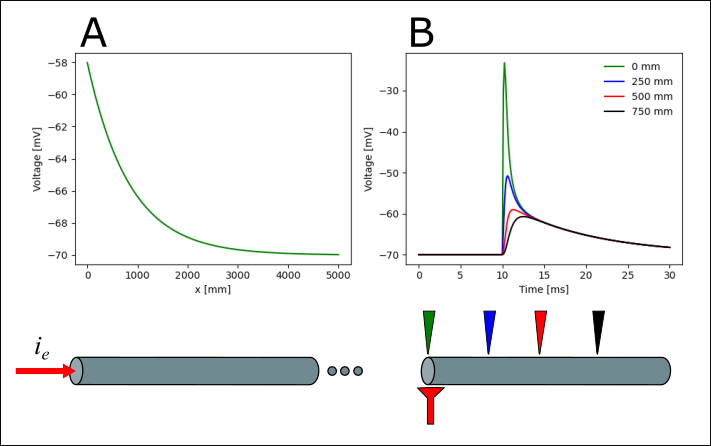
\includegraphics[width=0.7\textwidth]{Figures/Neuron/Cablesims.png}
\end{center}
\caption{\textbf{Stick-neuron responding to transient and constant inputs received in one end.} (A) Finite cable of length $L = 1 \, \si{\milli\metre}$ simulated numerically as 100 compartments, and stimulated with an alpha-synapse in the first compartment ($0<x<10 \, \si{\micro\metre}$). Transient responses shown at different distances from the synapse. The peak response decreases with distance from the synapse, and the time to reach the peak increases with distance from the synapse.
(A) Analytical steady-state solution for semi-infinite cable receiving a constant input $I_\text{stim} = 0.1 \, \si{\nano\ampere}$ in a sealed end at $x=0$. The membrane potential decays exponentially with distance from the stimulus site.  (A-B) Parameters choices: $c_\text{m}=1\, \si{\micro\farad\per\square\centi\metre}$, $d = 1\, \si{\micro\metre}$, $R_\text{a}=35.4\, \si{\ohm\centi\metre}$, $R_\text{m} = 10 \, \si{\kilo\ohm\square\centi\metre}$, which gives a length constant $\lambda = 840\, \si{\micro\metre}$.}
\label{fig:Neuron:Semiinf}
\end{figure}


%%%%%%%%%%%%%%%%%%%%
\subsection{\blue{Cable equation}}
\label{sec:Neuron:cableeq}
\index{Cable equation}
If we in \fref{eq:Neuron:multipassive} let $L \rightarrow \delta x$, and take the limit $\delta x \rightarrow 0$, we can derive the cable equation (see e.g., \cite**{Sterratt2011}): 

\begin{equation}
c_\text{m} \frac{\partial V}{\partial t} = \frac{E_\text{m}-V}{R_\text{m}} +  \frac{d}{4 R_\text{a}}  \frac{\partial^2 V}{\partial x^2}  + \frac{\mathcal{I}_{\mathrm{stim}}}{\pi d},
\label{eq:Neuron:cable}
\end{equation}
where we have introduced the stimulus current per unit length,
\ehnote{synes det er mindre kloenete aa definere denne som $I_\mathrm{stim}(x, t)$ i enhet A direkte. $\mathcal{I}_\mathrm{stim}(x,t)$ dukker jo bare opp en gang nedenfor for saa aa bli omdefinert til $I_\mathrm{stim}(x,t)$ igjen.} 
\begin{equation}
\mathcal{I}_{\mathrm{stim}}(x,t) = \lim_{\delta x \to 0} I_{\mathrm{stim}}(x,t)/\delta x \,\; (\si{\milli\ampere\per\centi\metre}). 
\label{eq:Neuron:CurrentPerUnitLength}
\end{equation}
To improve our analytical understanding of dendritic signaling, it is useful to reformulate the cable equation to:
\begin{equation}
\tau_\text{m} \frac{\partial V}{\partial t} = E_\text{m}-V +   \lambda^2  \frac{\partial^2 V}{\partial x^2}  + \frac{R_\text{m} \mathcal{I}_{\mathrm{stim}} }{\pi d},
\label{eq:Neuron:cable2}
\end{equation}
where we have multiplied all terms with $R_\text{m}$ and introduced the length constant \index{Length constant},
\begin{equation}
\lambda = \sqrt{\frac{d R_\text{m}}{4 R_\text{a}}} \,\; (\si{\centi\metre}), 
\label{eq:Neuron:lengthconst}
\end{equation}
and the time constant \index{Membrane time constant}, 
\begin{equation}
\tau_\text{m} \equiv R_\text{m} c_\text{m}  \,\; (\si{\milli\second}).
\label{eq:Neuron:timeconst}
\end{equation}
Here, $\tau_\text{m}$ is typical time scale (dimensionless time: $t/\tau$), while $\lambda$  is typical length scale  (dimensionless length: $x/\lambda$) for signals in the cable. If a certain point along the cable is perturbed, so that the potential is shifted from rest to a given value $V$, $\tau_\text{m}$ will determine how fast the local potential falls back towards rest, while $\lambda$ will tell us how far the local perturbation will spread along the cable. 

The cable equation is a continuous version of \fref{eq:Neuron:multipassive}. Whereas MC models generally must be solved numerically, the cable equation allows the spatiotemporal evolution of the membrane potential to be solved analytically for some idealized scenarios. Below, we consider a couple of scenarios that will  make the interpretation of $\tau_\text{m}$ and $\lambda$ clearer. 


%%%%%%%%%%%%%%%%%%%%
\subsection{\blue{Steady state solution of the cable equation}}
\label{sec:Neuron:cableSS}
\tvnnote{Bruker vi dette noe sted?}
Let us find the steady state solution for a semi-infinite cable, receiving a constant current injection at a sealed end in $x=0$ (\Fref{fig:Neuron:Semiinf}B). Since only the end-point receives the stimulus, we may attack this problem by solving \fref{eq:Neuron:cable2} for all other points $x>0$, and then introduce the stimulus current as a boundary condition. 

At steady-state, $\partial V/\partial t = 0$, and \fref{eq:Neuron:cable2} becomes:
\begin{equation}
0 = E_\text{m}-V +  \lambda^2 \frac{\partial^2 V}{\partial x^2}, 
\label{eq:Neuron:semiinf}
\end{equation}
at all points along the cable, except $x=0$. If we introduce the new variable $\Delta{V}=V-E_\text{m}$, \fref{eq:Neuron:semiinf} simplifies to:
\begin{equation}
\frac{d^2 \Delta{V}}{d x^2} -  \frac{1}{\lambda^2} \Delta{V}=0, 
\label{eq:Neuron:semiinf2}
\end{equation}
which has the solution:
\begin{equation}
\Delta{V}(x) = \Delta{V}(0) e^{-x/\lambda}, 
\label{eq:Neuron:semiinf3}
\end{equation}
or, 
\begin{equation}
V(x) = E_\text{m} + \big( V(0)-E_\text{m} \big) e^{-x/\lambda}.
\label{eq:Neuron:semiinf4}
\end{equation}
We note that the general-solution to \fref{eq:Neuron:semiinf2} also has a term containing $e^{+x/\lambda}$, but this was excluded on the count of being unphysical, since it diverges when $x \rightarrow \infty$. 

To obtain the final solution of the problem, we need to specify the boundary value $V(0)$, which will depend on the stimulus current. Since the stimulus is injected in a singular point ($x=0$), we go back to expressing in terms of a total current, $I_\text{stim}$ (and not as a current per unit length $\mathcal{I}_\text{stim}$). We can introduce it through a boundary condition demanding that the injected current must be identical to the axial current in the cable at $x=0$:
\begin{equation}
I_\text{stim} = - \frac{\pi d^2}{4}\frac{1}{R_\text{a}} \frac{\partial V}{\partial x}   \Big|_{x=0}.
\end{equation}
If we insert for $\partial V/\partial x$ (calculated from \fref{eq:Neuron:semiinf4}), and insert \fref{eq:Neuron:lengthconst} for $\lambda$, we can derive the following expression for $V(0)$:
\begin{equation}
V(0) = E_\text{m} + R_{\infty}I_\text{stim}, 
\label{eq:Neuron:firstRinf}
\end{equation}
where we have defined:
\begin{equation}
R_{\infty} = \sqrt{\frac{R_\text{m} R_\text{a}}{\pi^2 d^3}}.
\label{eq:Neuron:Rinf}
\end{equation}
If we now insert \fref{eq:Neuron:firstRinf} into \fref{eq:Neuron:semiinf3}, we obtain our final solution:
\begin{equation}
V(x) = E_\text{m} +R_{\infty}I_\text{stim}  e^{-x/\lambda}.
\label{eq:Neuron:semiinf4}
\end{equation}

The steady state solution to the semi-infinite cable (plotted in \Fref{fig:Neuron:Semiinf}B) is useful as it gives us analytical insight into signals spreading in e.g., passive dendrites. Some insights that can be derived from it is:

\begin{itemize}

\item It follows from \fref{eq:Neuron:firstRinf} that $R_{\infty} = (E_\text{m}-V(0))/I_\text{stim}$, and thus interprets as the steady-state input resistance of the semi-infinite cable. \Fref{eq:Neuron:Rinf} thus shows that the input resistance is proportional to $1/d^{3/2}$, i.e., the input resistance is higher the thinner the dendrite. 

\item \Fref{eq:Neuron:semiinf4} shows that in steady-state, the amplitude will decay exponentially from the injection site and outwards, and will be reduced by a factor $1/e$ over the length $\lambda$. If we insert some typical values into \fref{eq:Neuron:lengthconst}, like a dendritic diameter of $d=1 \, \si{\micro\metre}$, a membrane resistance of $R_\text{m}=10 \,
\si{\kilo\ohm\square\centi\metre}$, and an axial resistivity $R_\text{a}=35.4\, \si{\ohm\centi\metre}$\tvnnote{litt lavt?}\ehnote{ikke for giant squid}, we get a length constant of $\lambda = 840\, \si{\micro\metre}$. Dendrites with lengths in this order will thus only be moderately affected by the membrane potential in the soma.

\item According to \fref{eq:Neuron:lengthconst}, $\lambda \propto \sqrt{d}$, meaning that signals will spread further the thicker the dendrite.

\item According to \fref{eq:Neuron:lengthconst}, $\lambda \propto \sqrt{R_\text{m}/R_\text{a}}$ meaning that the signal is facilitated by having a large membrane resistance compared to axial resistance. 
\end{itemize}


\subsection{\blue{GH: Temporal solutions of cable equation}}
\label{sec:Neuron:cabletemp}
\tvnnote{Bruker vi dette noe sted?}
In \fref{fig:Neuron:Semiinf}A we simulated numerically the response of a cylindrical neuron to a  synaptic input in one end. It is possible to show analytically that the passive decay of $V$ following the input-induced peaks can be expressed as a sum of exponentials \cite**{rall1969}:
\begin{equation}
V(x,t) = C_0(x) e^{-t/\tau_0} + C_1(x) e^{-t/\tau_1} + C_2(x) e^{-t/\tau_2} + \ldots, 
\label{eq:Neuron:cabletemporal}
\end{equation}
where the coefficients $C_n(x)$ depend on the distance along the cable, while $\tau_0 = \tau_\text{m} = R_\text{m} c_\text{m}$ is the \emph{membrane time constant} (\fref{eq:Neuron:timeconst}), and the other time constants have successively smaller values ($\tau_0 > \tau_1 > \tau_2 > \ldots$). We will not here present these analytical results in any further detail, but note that the final decay phase, i.e., when $V$ at all locations have coincided, takes place at the slower time scale of the membrane time constant, $\tau_\text{m}$ which in the simulation in \Fref{fig:Neuron:Semiinf}A  was 10 \si{\milli\second} ($R_\text{m}=10\,\si{\kilo\ohm\square\centi\metre}$, and $c_\text{m}=1\, \si{\micro\farad\per\square\centi\metre}$). 


\subsection{\blue{Frequency dependence of the cable length constant}}
\label{sec:Neuron:cablefreq}
\tvnnote{Kanskje velge et mer generelt navn? }
As we just saw, the length constant $\lambda$ (\fref{eq:Neuron:lengthconst}) is the length over which the potential falls to a fraction $1/e$ of its boundary value when the finite end of a semi-infinite cable is fixed at a constant potential, or, equivalently, if the end of a semi-infinite cable receives a constant direct-current (DC) input. Therefore, $\lambda$ is often referred to as the DC length constant. 

It is possible to derive a corresponding length constant for AC input to a semi-infinite cable \cite**{Pettersen2008a}: 
\begin{equation}
\lambda_{AC} = \lambda \sqrt{ \frac{2}{1+\sqrt{(\omega \tau)^2 + 1}} }.
\label{eq:Neuron:AClambda}
\end{equation}
Here $\tau$ \ehnote{$\tau_\mathrm{m}$?} still is the membrane time constant (\fref{eq:Neuron:timeconst}), $\lambda$ is still the DC length constant (\fref{eq:Neuron:lengthconst}), and $\omega = 2\pi f$ is the angular frequency of the the boundary potential.

For a constant boundary condition ($I_\text{stim} = \text{constant}$ in \fref{eq:Neuron:semiinf4}) or, equivalently, $V(0) = \text{constant}$ in \fref{eq:Neuron:semiinf3}), $\omega$ is zero, and we may verify that $\lambda_{AC}$ becomes identical to the DC length constant $\lambda$. For an AC input, we see that $\lambda_{AC}$ decreases with $\omega$, and for high frequencies $\lambda_{AC} \propto (\omega \tau^{-1/2})$. Thus, low frequency input will tend to travel further in dendritic structures, while high frequency input will only affect dendritic structures more locally. 

When a neuron receives an input current (synaptic or injected) in a particular point, the same amount of current will have to leave the neuron from other points along the neural extension. The spatial separation between the input current (sink) and return currents (sources) will be proportional to the neuronal length constant, and from \fref{eq:Neuron:AClambda} we thus know that the source/sink separation will be larger for low frequency components of the neuronal activity. As we shall see later, the spatial separation between inward (sinks) and outward (sources) transmembrane currents is an important factor determining the size and shape of extracellular potentials. 
\tvnnote{Har skrevet om dette i LFP-kapittelet ogsaa, kanskje slaa sammen?}
\ehnote{Jeg tenker vi ikke trenger aa spekulere om effekten paa EPs her.}



%%%%%%%%%%


\section{\blue{Ion concentration dynamics and reversal potentials}}
\label{sec:Neuron:Ions_and_reversals}
\index{Ion concentration dynamics}
MC models as defined in \fref{sec:Neuron:Active_multicomp} with membrane mechanisms as specified in \fref{sec:Neuron:membranecurrents} give a complete and operational framework for modeling the electrical activity of neurons, and works well for most purposes. The reader may chose to skip the remainder of this chapter, which delves more into the biophysical origin of neural activity. 

Up til this point, we have focused on electrical currents in neurons, but talked little of their biophysical origin, i.e., the ions that carry these electrical currents. For example, action potentials are generated by a transmembrane influx of Na\textsuperscript{+}, 
which charges up \ehnote{dropp "up" -- antonymet til "discharge" er vel bare "charge"?}
(depolarizes) the neuron, followed by an efflux of K\textsuperscript{+}, which discharges (repolarizes) it. These fluxes are primarily driven by diffusion, and thus depend on the intra- and extracellular solutions having different ionic compositions. 

In the MC models it is normally assumed that, despite all these various ionic fluxes, the ion concentrations remain constant. This may seem like a peculiar assumption, but it is often quite good. The reason is that the number of ions crossing the membrane during a brief signal such as an action potential only leads to tiny changes in the ion concentrations. 

To see why, let us consider an example with a spherical single compartment neuron with radius $r$. This neuron will contain a number $N_0 = 4/3 \,\pi r^3 N_\text{A} c_\text{Na}$ of Na$^{+}$ ions, where $N_\text{A}$ is Avogadro's number and $c_\text{Na}$ the intracellular Na$^{+}$ concentration. Let us next assume that Na$^+$ ions enter the neuron and increases the membrane potential by $\Delta V$. The total charge needed for this will be $\Delta Q = 4 \pi r^2 c_m \Delta V$, which corresponds to a number of $N_\text{new} = \Delta Q/e$ of ions, where $e$ is the unit charge. From this, we may compute the ratio between the number of ions that entered the neuron and the number of ions that were already there:
\begin{equation}
\frac{N_\text{new}}{N_0} = \frac{3 c_m \Delta V}{F r c_\text{Na}}, 
\label{eq:Neuron:NaNaNa}
\end{equation}
where we have used that Faraday's constant $F = eN_\text{A} = 96458.3 \, \si{\coulomb\per\mol}$. If we insert values for a typical action potential $\Delta V = 100 \,\si{\milli\volt} = 0.1 \si{Volt}$, an intracellular Na$^+$ concentration $c_\text{Na} = 10 \, \si{\milli\molar}$, and $c_\text{m} = 1 \, \si{\micro\farad\per\square\centi\metre} = 10^{-2}\, \si{\farad\per\square\metre}$, the ratio becomes:
\begin{equation}
\frac{N_\text{new}}{N_0} = \frac{3.1 \times 10^{-9} \si{\metre}}{r}, 
\label{eq:Neuron:NaNaNaNa}
\end{equation}
Hence, even in a small compartment with $r=1\,\si{\micro\metre} = 10^{-6}\,\si{\metre}$, the number of ions that enters during an action potential will only change the concentration by fraction $3.1 \times 10^{-3} \approx 0.3 \%$. This suggests that concentrations changes on a short time scale are small enough to be neglected. 
\tvntxt{It also serves to demonstrate how relatively tiny the deviations from electroneutrality across the membrane are, while still giving rise to substantial membrane potentials.}\tvnnote{Vet ikke helt om dette er riktig?}

Since neurons possess a team of homeostatic mechanisms that strive to maintain the trans-membrane ion concentration gradients, the assumption of constant ion concentrations also tends to hold on a longer time scale. The perhaps most important of these mechanisms is the ATPase pump, which uses \tvntxt{the} energy \tvntxt{of 1 ATP molecule} to pump \tvntxt{2} K$^+$ ions into the neuron and \tvntxt{3} Na$^+$ ions out, thus reversing the ionic exchange that occurs during action potential generation. As a result of this pump, the intracellular space tends to remain comparatively rich in K$^+$, while the extracellular space is tends to remain comparatively rich on Na$^+$. Typical values of ion concentrations of the main charge carriers inside and outside neurons are given in \Fref{tab:Neuron:ion-concentrations}. 

\begin{table}[h]
%\centering
\caption[]{Major charge carrier concentrations inside/outside a typical mammalian neuron. Concentration values were taken from Table 2-1 in \citeasnoun**{Somjenboka} for neurons in the central nervous system (intracellular) and human cerebrospinal fluid (extracellular). Values vary with species and brain regions. Nernst potentials were computed from \fref{eq:Neuron:revpots} assuming a body temperature of 309.15 \si{\kelvin}.
}
\label{tab:Neuron:ion-concentrations}
\begin{tabular}{@{}lcccccc@{}}
\hline
					& 	K$^+$	&	Na$^+$	&	Mg$^{2+}$	  &	Cl$^-$	&	Ca$^{2+}$	 	& HCO3$^-$ 	\\ 
\hline
Intracellular (\si{\milli\molar})	 	   & 125		&		10	&		0.5	&	6.6		&  	6$\times$10$^{-5}$	  & 	18 \\
Extracellular (\si{\milli\molar})			           & 2.9			&		147	&		0.7	&	119 		&		1	&	23.3	  	\\
Nernst potential (\si{\milli\volt})		    &	-100		&	    	+72	&		+4.5	&	-77		&		+129 	& 	-6.9  	\\
\hline
\end{tabular}
\end{table}

In HH-type models, the ensemble of processes that work to maintain baseline conditions are simply assumed to do their job, and not explicitly modeled. Instead, they are grouped together into the \textit{passive} leakage current $I_\text{L}$ (\fref{eq:Neuron:HHleak}), which largely determines the cell's resting potential (see see \cite**{offner1991} for a critical study of this approximation). \tvnnote{Kan virke litt som vi antyder at ione-pumpene er inkludert i leak current syntes jeg. Flytte dette til begynnelsen av neste subsection?} Below, we shall explain how the ionic concentrations are implicitly present in the HH-formalism as they determine the ionic reversal potentials ($E_x$ in \fref{eq:Neuron:HHform}). We shall also comment briefly on the cases where the assumptions of constant ion concentrations are not applicable. 


\subsection{\blue{Ionic reversal potentials}}
\label{sec:Neuron:Erev}
\index{Reversal potential}
Ion channels are pores in the membrane, some of which are selectively permeable only to specific ions. The ion flux through an open ion channel will be mediated by a combination of (i) diffusion and (ii) electric drift as predicted from the Nernst-Planck equation (\fref{eq:Basics:JNP}).

The ionic reversal potential \index{Reversal potential} is defined as the membrane potential at which the diffusive and drift currents of a given ion species are in an equilibrium, i.e., they are equal in magnitude but oppositely directed. If we approximate the membrane currents as one-dimensional (in the $z$-direction, perpendicular to the membrane), the Nernst-Planck equation for an ion species $k$ is:

%%%%
\begin{equation}
j_k = j_{k,\text{diff}} + j_{k,\text{drift}} 
=  - P_k \Big(\frac{d[k]}{dz} +  \frac{Fz_k}{RT}  [k] \frac{dV}{dz} \Big), 
\label{eq:Neuron:NP1D}
\end{equation}
%%%%
where the first term \tvntxt{inside the parenthesis} is Fick's law for the diffusive flux density along the concentration gradient, and the second term is the electrical drift along the voltage gradient. 
\ehtxt{[k] denotes the concentration of ion $k$ (\si{\molar\per\metre^3}).}
Since we consider membrane fluxes, we have replaced the diffusion constant ($D_k$) which appears in the more common form of the Nernst-Planck equation (\fref{eq:Basics:JNP}) with the membrane's permeability ($P_k$) to ion $k$. The reversal potential (also called the Nernst-potential) is found by solving for when there is no net flux, i.e., when  $j_{k,\text{diff}} = - j_{k,\text{drift}}$:

\begin{equation}
\frac{1}{[k]} \frac{d[k]}{dz} = - \frac{Fz_k}{RT}  \frac{dV}{dz}.
\end{equation}
We may multiply both sides by $dz$ and re-arrange this to get:
\begin{equation}
-dV = \frac{RT}{Fz_k}  \frac{d[k]}{[k]}.
\end{equation}
If we integrate this from the inside to the outside of the membrane, we get:
\begin{align}
-\int_{V_{\text{in}}}^{V_{\text{out}}}  dV &= \frac{RT}{Fz_k}  \int_{[k]_{\text{in}}}^{[k]_{\text{out}}} \frac{d[k]}{[k]} \rightarrow \\
V_{\text{in}}-V_{\text{out}} &= \frac{RT}{Fz_k} ln \frac{[k]_{\text{out}}} {[k]_{\text{in}}} \rightarrow \\
E_k & =  \frac{RT}{Fz_k}  ln \frac{[k]_{\text{out}}} {[k]_{\text{in}}} 
\label{eq:Neuron:revpots}
\end{align}
where the last equality follows from the definition of $E_k$ as the membrane potential $V_{\text{in}}-V_{\text{out}}$ for which the the net flux (in \fref{eq:Neuron:NP1D}) is zero. \Fref{eq:Neuron:revpots} was used to compute the reversal potentials listed in \Fref{tab:Neuron:ion-concentrations}. 

To illustrate how to interpret the reversal potential, we can use a K$^+$ channel as an example. For simplicity, let us assume that it opens at a time when the neuron is resting ($V = V_{\text{in}}-V_{\text{out}} \sim -70 \, \si{\milli\volt}$), and that the K$^+$ is the only ion channel that opens. Since the intracellular space is more K$^+$-rich than the extracellular space, diffusion will drive K$^+$ out from the neuron, and since $V$ is negative, electric drift will drive K$^+$ into the neuron. Initially, the diffusive process will dominate, so that there will be a net efflux of K$^+$. This will cause a gradual decrease (hyperpolarization) of $V$ towards the K$^+$ reversal potential, which with concentrations as in \fref{tab:Neuron:ion-concentrations} has the value $E_K = -100 \, \si{\milli\volt}$. As $V$ decreases, the drift component will become stronger, and when $V$ reaches $E_K$, it becomes equal in magnitude to the diffusive component, and the net K$^+$ current becomes zero. $E_K$ is called the reversal potential, because if the potential were to drop below this value, the current would reverse, i.e., the drift component would become dominant over diffusion, and K$^+$ would start to go inward into the neuron. 

As ion concentrations are generally assumed to remain constant in HH-type models, the reversal potentials are also assumed to be constant. As a consequence, one typically does not worry about ionic concentrations when constructing such models, but simply uses values for $E_k$ based or empirical measurements of the potential at which a certain membrane current reverses.


\subsection{\blue{The Goldman-Hodgkin-Katz equation}}
\label{sec:Neuron:GHK}
\index{Goldman-Hodgkin-Katz equation}
\Fref{eq:Neuron:NP1D} defined the reversal potentials for individual ion species, and is relevant for modeling ion-specific ion channels. To calculate the reversal potential for a non-specific ion channel, we need to express all the individual ion currents separately, and compute the value of $V$ for which they sum to zero. 

If we combine \fref{eq:Neuron:NP1D} with the assumptions that (i) ions cross the membrane independently, and (ii) that the electric field within the membrane is constant, we can derive the Goldman-Hodgkin-Katz (GHK) equation for the membrane currents (see e.g., \cite**{hodgkin1949,johnston1994foundations}):
\begin{equation}
I_\text{k} = P_k z_k F \frac{z_k F V}{R T} \Big( \frac{[k]_\text{in}-[k]_\text{out} e^{-z_k F V/RT}} {1-e^{-z_k F V/RT}} \Big).
\label{eq:Neuron:GHK}
\end{equation}

An example of a non-specific ion channel is the passive leakage current which has a permeability to all ion species simultaneously, so that its reversal potential ($E_\text{L}$ in \fref{eq:Neuron:HHleak}) will depend on all ion concentrations. If we assume that only the three most abundant charge carriers (K$^{+}$, Na$^{+}$ and Cl$^{-}$) contribute, and that they have leak permeabilities $P_\text{K}$, $P_\text{Na}$ and $P_\text{Cl}$, we can derive from \fref{eq:Neuron:GHK} that they are in equilibrium at the potential:
\begin{equation}
E_\text{L} = \frac{R T}{F} 
\ln \frac{P_\text{K} [\text{K}_\text{out}+P_\text{Na} [\text{Na}]_\text{out} + P_\text{Cl} [\text{Cl}l]_\text{in}}
           {P_\text{K} [\text{K}]_\text{in}+P_\text{Na} [\text{Na}]_\text{in} + P_\text{Cl} [\text{Cl}]_\text{out}}.
\label{eq:Neuron:Eleak_GHK}
\end{equation}

Looking at \fref{eq:Neuron:GHK}, we see that the transmembrane currents are nonlinear functions of both the ionic concentrations $[k]$ in the intra and extracellular space, and the membrane potential $V$. In comparison, the transmembrane currents used in the HH-type formalism (\fref{eq:Neuron:HHform}), assumed to be proportional to the driving force $(V-E_k)$, are linearized (sometimes called quasi-Ohmic) versions of the Goldman-Hodkgkin-Katz equation. The HH-form (\fref{eq:Neuron:HHform}) is generally deemed as sufficient for modeling most ion channels, because it gives good predictions of the membrane currents. Ion concentrations and ionic reversal potentials are then assumed to be constant.


\subsection{\blue{Intracellular Calcium dynamics}}
\label{sec:Neuron:Calcium}
\index{Calcium dynamics}
While most ion concentrations are assumed to be constant in HH-based models,
\ehnote{mer riktig aa si "... constant in models utilizing the HH formalism,"}  
it is common to make an exception for Ca$^{2+}$. The main reason for this is that the intracellular Ca$^{2+}$ concentration ($\mathrm{[Ca]_i}$) is very low compared to that of the other ion species (\Fref{tab:Neuron:ion-concentrations}). Unlike for the other ion species,  $\mathrm{[Ca]_i}$, can therefore change quite dramatically on a short time scale, for example during the opening of Ca$^{2+}$ channel. 

The motivation for explicitly keeping track of changes in $\mathrm{[Ca]_i}$ are several. Firstly, to accurately model currents through Ca$^{2+}$ channels, the concentration-dependent GHK formalism (\fref{eq:Neuron:GHK}) is often used (see e.g., \cite**{Destexhe1994,Zhu1999,Halnes2011}), and one then needs to simulate $\mathrm{[Ca]_i}$. Secondly, modeling $\mathrm{[Ca]_i}$ could be motivated by the aim to reproduce data from Ca$^{2+}$ imaging experiments. Thirdly, Ca$^{2+}$ does not only act as a charge carrier in neurons, but is also a second messenger, which means that it can trigger a number of intracellular chemical processes, including the gating of Ca$^{2+}$ activated ion channels. 

When Ca$^{2+}$ dynamics is included in HH-based models, it is usually to account for the activation of ion channels that instead of being voltage gated, open or close as a function of $\mathrm{[Ca]_i}$\index{Calcium-gated ion channels}. The kinetics scheme for voltage gated ion channels (\fref{eq:Neuron:HHgate}) is then replaced with one dependent on $\mathrm{[Ca]_i}$:

\begin{equation}
\frac{dx(V,t)}{dt} = \frac{x_{\infty}(\mathrm{[Ca]_i}) - x}{\tau_x(\mathrm{[Ca]_i}},  \, \text{for } x = \{m,h\},
\label{eq:Neuron:Cagate}
\end{equation}
and the $\mathrm{[Ca]_i}$ in a neuronal compartment is typically modeled using a simplified framework on the form:
\begin{equation}
\frac{d\mathrm{[Ca]_i}}{dt} = \gamma i_{\text{Ca}} - \frac{\mathrm{[Ca]_i}-\mathrm{[Ca]_{i,0}}}{\tau_{Ca}}, 
\label{eq:Neuron:Cadynamics}
\end{equation}
where a transmembrane Ca$^{2+}$ current ($i_\text{Ca}$ is converted to a change in $\mathrm{[Ca]_i}$ by the conversion factor $\gamma$, which is proportional to the surface to volume ratio of the neuronal compartment where $\mathrm{[Ca]_i}$ is defined. In addition, the last term in \fref{eq:Neuron:Cadynamics} represents the summed activity of a number of extrusion mechanisms that will make $\mathrm{[Ca]_i}$ decay towards some baseline value $\mathrm{[Ca]_{i,0}}$ with a time constant $\tau_\text{Ca}$ (see e.g. \cite**{Sterratt2011}).

To use a simple model as in \fref{eq:Neuron:Cadynamics} might not be meaningful when it comes to model the more abundant ion species (K$^{+}$, Na$^{+}$ and Cl$^{-}$). One reason is that \fref{eq:Neuron:Cadynamics} only considers the intracellular concentration. This makes sense for Ca$^2+$, since the intracellular concentration is much smaller than the extracellular concentration, so that dramatic relative changes of $\mathrm{[Ca]_i}$ can occur without requiring correspondingly dramatic relative changes in the extracellular concentration. The same does not hold for the more abundant species, for which the concentrations are of the same order of magnitude on both sides of the membrane. Another reason is that \fref{eq:Neuron:Cadynamics} is local in the sense that the concentration is affected exclusively by transmembrane ionic currents. In reality, also the axial intracellular currents are carried by ions, especially by the more abundant ones \cite**{Qian1989}. A complete and consistent model of ion concentration dynamics would thus need to account for electrodiffusive ion concentration dynamics both in the intra- and extracellular space. Such models exist (see e.g., \cite**{Saetra2020,ellingsrud2020}), but they are generally computationally heavy, and not based on the MC framework that we have presented here. 


\section{\blue{Underlying assumptions in multicompartment models}}
\label{sec:Neuron:HHCassumptions}
Like any model, MC type models are simplified representations of the real system, and rest on a series of simplifying assumptions. Since MC type models with HH-type ion channels have become quite a pillar in modern neuroscience, their weaknesses and general applicability have been the subject of numerous publications within the field (see e.g., \cite**{Rinzel1990,Meunier2002,Catterall2012,Almog2016,Drukarch2018}). We will not give any detailed discussion on this topic here, but we will briefly just list up the main assumption that MC models rest upon. 

\begin{itemize}
\item \textit{Cable equation}: MC models rest on the assumption that neuronal morphology is well represented by a one-dimensional, branching cable. As such, MC type models neglect the radial components of intracellular currents (see e.g.,\citeasnoun**{lindsay2004maxwell} for a critical study of this approximation).

\item \textit {Ion channels}: HH-type ion channels are simplified approximations of the electrophysiological dynamics of ion channel gating. Since the HH-type formalism is based on deterministic equations, it cannot account for ion channel noise, which can stem from the stochastic gating at the single channel level \cite**{Meunier2002, Goldwyn2011}. Furthermore, the relatively simple gating kinetics described by HH-type channels is not accurate for all ion channels, and more detailed ion channel models have been developed, based on a formalism more compatible with statistical physics and thermodynamics \cite**{Destexhe2010}, or even more detailed, Markov-type formalism based on single-channel recordings \cite**{sakmann2013}.

\item \textit{Ion concentrations}: As we explained in \fref{sec:Neuron:Ions_and_reversals}, the concentrations of the main charge carriers are in standard MC models assumed to be constant. As the main ion concentrations change little during normal neuronal activity, this assumption is often warranted. However, there exist scenarios when this is not true, and dramatic changes in ion concentrations is a trademark of several pathological conditions, such as epilepsy, stroke and spreading depression \cite**{Somjen2001,Zandt2015,Ayata2015}. Effects of changes in ion concentrations on the dynamical properties of neurons has been the topic of many modeling studies (see e.g., \cite**{Qian1989,Kager2000,Ullah2009,Zandt2011,Wei2014,WeiUllahSchiff2014,Hubel2014,Saetra2020}), but are not accounted for by standard MC models.

\item \textit {Ephaptic effects}\index{Ephaptic effects}: While direct neural communication is mediated through chemical and electrical synapses, a neuron can also affect neighboring neurons indirectly by altering the extracellular environment, either through its exchange of ions with the surroundings, or through the electric fields that it generates \cite**{Jefferys1995}. These indirect effects are often referred to as \textit{ephaptic coupling}. 
In principle, a neuron can also affect itself (\textit{self-ephaptically}) by changing its own extracellular environment \cite**{Roth1994}.\tvnnote{Jeg visste ikke at endringer i konsentrasjon kunne kalles 'ephaptic', jeg trodde dette kun gjalt ekstracellulaere felt?}

Being based on the assumption that ion concentrations do not vary and the extracellular space being grounded ($V_e = 0$ \ehnote{$V_\mathrm{e}$?} in \fref{eq:Neuron:multimain}), 
MC models do not account for ephaptic effects. The main argument for neglecting ephaptic concentration effects is, as we have explained earlier, that concentrations tend to remain relatively constant under most circumstances. The main argument for neglecting electric ephaptic effects is that $V_e$ generally is much smaller than the membrane potential $V$, and therefore not likely to affect it notably. Self-ephaptic effects have been accounted for in simulations by using the two-step scheme (\Fref{sec:Basics:twostep}) interatively \cite**{Gold2006}, i.e., first (i) used MC models to compute $V$ assuming $V_e = 0$, next (ii) use volume conductor (VC) theory to compute $V_e$, and then (iii) refine the estimates in (i) by accounting for the effects of $V_e$ on $V$. According to \citeasnoun**{Gold2006} this did not significantly affect the numerical results\tvnnote{Gold siterer bare Holt1998 paa dette, og Holt1998 sier han har testet men viser ingenting. Jeg testet dette litt selv i LFPy, og det var ingen nevneverdig effekt. Ha med figur om dette?}. However, electric ephaptic coupling between different neurons have been suggested to play a possible role, for example in brain regions with low extracellular conductivity, or in bundles of axons \cite**{Holt1999,Bokil2001,anastassiou2015,Goldwyn2016,Tveito2017,Shifman2019}. Such effects are not accounted for in the standard MC models.

Importantly, the negligence of ephaptic effects when using the two-step scheme is implicit in the way that the neurons are modeled (Step 1), but not part of the physical fundament of the VC theory (Step 2) used to compute extracellular potentials. VC theory does not in itself make any assumption regarding ephaptic effects being present or not. Hence, the the extracellular potential should satisfy \fref{eq:Basics:continuity2} regardless of whether or not ephaptic effects were accounted for when the neural current sources $C$ were computed. 
\ehnote{Variabelen $C$ kan vel kanskje utelates her.}
As our main focus is on the extracellular potential, we will therefore stick with the two-step scheme throughout most of this book.
\end{itemize}